\documentclass[tikz,border=5]{standalone}
\usetikzlibrary{matrix,arrows.meta}
\usepackage{tikz-cd}
\usetikzlibrary{arrows,calc}
\usepackage{xypic}
\begin{document}


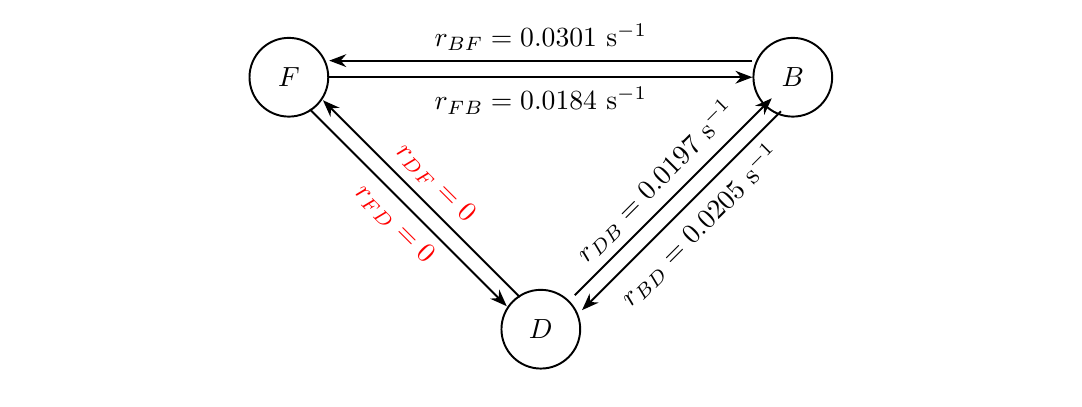
\begin{tikzpicture}[>=Stealth,->,line width=.7pt]
\matrix [matrix of math nodes,
column sep={3.2cm,between origins},
row sep={3.2cm,between origins},
nodes={circle, draw, minimum size=1cm}]
{
& |(1)| F &   & |(2)| B & \\
&  & |(3)| D & \\};

\draw [transform canvas={xshift=0pt,yshift=0pt}] (1)--(2) node [midway, below] {$r_{FB}=0.0184~{\rm s}^{-1}$}; 
\draw[transform canvas={xshift=0pt,yshift=6pt}] (2)--(1) node [midway, above] {$r_{BF}=0.0301~{\rm s}^{-1}$};



\draw[transform canvas={xshift=2pt,yshift=2pt},shorten <= -1pt]  (3)-- (1)  node[midway, above,sloped] {$\color{red} r_{DF}=0$};
\draw[transform canvas={xshift=-2pt,yshift=-2pt},shorten <= -1pt] (1)--(3)
node[midway, below,sloped] {$\color{red}r_{FD}=0$};

\draw[transform canvas={xshift=2pt,yshift=2pt},shorten >= -1pt] (3)--(2) node[midway, left,above, sloped] {$r_{DB}=0.0197~\mathrm{s}^{-1}$};;
\draw[transform canvas={xshift=6pt,yshift=-2pt},shorten >= -2pt] (2)--(3) node[midway, below,sloped] {$r_{BD}=0.0205~ \mathrm{s}^{-1}$};

\end{tikzpicture}
\end{document}
